\chapter{7 TeV and 8 TeV Differential Cross Section Measurement: Data, Simulation and Selection}
\label{c:Differential_Cross_Section:data_simulation_and_selection}

\section{Introduction}
\label{s:analysis1_introduction}
This analysis measures the normalised differential \ttbar cross section in the semi-leptonic channel and is
carried out on 2011 and 2012 data recorded from the CMS detector. The measurement is carried out with respect
to the following global, or primary, variables is carried out:
\begin {itemize}
  \item {\met, the missing transverse energy in an event}
  \item {\HT, the sum of the jet transverse momenta in an event}
  \item {\st, the sum of the observed transverse momenta in an event}
  \item {\mt, the transverse mass of the leptonically decaying \W boson}
  \item {\wpt, the transverse momentum of the leptonically decaying \W boson}
\end{itemize}

TODO:INCLUDE MT? %TODO: include MT?

Previous analyses using 7\TeV data investigating \met and using 8\TeV data investigatin all the
global variables listed above can be found in \cite{CMS-PAS-TOP-12-019} and \cite{CMS-PAS-TOP-12-042} respectively.

This investigation is motivated primarily by the importance of understanding \ttbar events since they are a
significant background in many new physics analyses. It is also helpful in understanding QCD and event
generators. Rare Standard Model processes such as $\ttbar + W\rightarrow l\nu$ or $\ttbar + Z\rightarrow
\nu\bar{\nu}$ would appear in \met distribution tail, and $\ttbar + X$ where $X$ is massive would appear in
the \HT and \st distributions. There are also possible new physics scenarios such as stop pair production,
$\tilde{t}\bar{\tilde{t}} \rightarrow t\tilde{\chi_0} \bar{t}\bar{\tilde{\chi_0}}$ which could show
hints of dark matter.

\section{Data and Simulated Samples}
\label{s:data_and_simulated_samples}

\subsection{Data}
\label{ss:data}

Data collected in 2011 at a centre-of-mass energy of 7\TeV and in 2012 at a centre-of-mass energy of
8\TeV are used. The datasets are determined by the triggers that were used to record them. For 7\TeV, the ElectronHad
dataset is used in the electron channel. It was recorded with triggers that select based on a single, isolated
electron and additional jets. At 8\TeV, the SingleElectron dataset was used for the electron channel
which is based on a single, isolated electron. In the muon channel, the SingleMu dataset was used for both
centre-of-mass energies, requiring a single, isolated muon. See Section~\ref{s:selection} for more
details about triggers. The datasets used are shown in Tables~\ref{tab:datasets7TeV} and {tab:datasets8TeV} in
Appendix~\ref{as:datasets}. Only data that is certified as “golden”, which is defined as data taken with the
detector working without any major faults, used. The masks used to filter out data taken in other periods are
specified in Table~\ref{tab:JSONfiles} in Appendix~\ref{as:datasets}.

\subsection{Simulated Samples}
\label{ss:simulated_samples}
The Monte Carlo generators used in this analysis are \MADGRAPH \cite{madgraph5}, \PYTHIA \cite{pythia8},
\POWHEG \cite{powheg_Nason,powheg_Frixione,powheg_Alioli}, HERWIG \cite{herwig} and MC$@$NLO
\cite{mcatnlo_Frixione1, mcatnlo_Frixione2}.

The signal for this analysis is the production of a \ttbar pair which decays semi-leptonically, \ie each of
the t quarks decays to a \W boson and a b jet, with one of the \W bosons decaying hadronically to two jets and
the other decaying leptonically to a lepton (electron or muon) and an associated neutrino.
Section~\ref{s:top_physics_at_the_lhc} outlines the signal and background events considered.

Additional, lower energy jets, can be produced from other scatterings in the same proton-proton interaction
and from gluon radiation from quarks in the decay. 

Tables~\ref{tab:signaldatasets7TeV} and \ref{tab:backgrounddatasets7TeV} show the Monte Carlo signal and
background samples respectively used in this analysis. Top pair production is modelled using \MADGRAPH, single
top events are modelled with \POWHEG, \W and \Z boson plus jets production is modelled using \MADGRAPH and QCD
multi-jet events are modelled with \PYTHIA. In all cases, \PYTHIA is used to model radiation and hadronisation
processes. Tables~\ref{tab:7TeVsystematicdatasets} and \ref{tab:8TeVsystematicdatasets} show the samples used
to evaluate the factorisation scale and matching threshold uncertainties. \WpJets and \ZpJets samples were not
made available at 7\TeV, so the scaled distributions from \SI{8}{\TeV} were used, as described in
Section~\ref{ss:7TeV_vjets_theory_systematic_template}.

\begin{table}[hbth]
\centering
\caption{\SI{7}{\TeV} Monte Carlo signal datasets used for this analysis.}
\label{tab:signaldatasets7TeV} \small\addtolength{\tabcolsep}{-5pt}
\begin{tabular}{llrrr}
%\multicolumn{6}{c}{Signal datasets}
%\hline
Process & Generator & $\sigma$ ($\pb$) & No. events & \lumiint ($\fbinv$) \\
\hline
\ttbar & \MADGRAPH & 177.31 & 17100187 & 96.4 \\
\ttbar & \MCATNLO & Not Available & - & - \\
\ttbar & \POWHEG-\PYTHIA & 177.31 & 4833135 & 27.3 \\
\ttbar & \POWHEG-\HERWIG & 177.31 & 4480816 & 25.3 \\
\hline
\end{tabular}
\end{table}


\begin{table}[hbth]
\centering
\caption{\SI{7}{\TeV} Monte Carlo background datasets used for this analysis. All samples are generated
inclusively if not marked otherwise ($^\star$ generator cut on in-flight-decays of b- and c-hadrons, $^\ominus$ enriched in conversion electrons; $l$ means
all leptonic decays: $l=e,\mu,\tau$; $^\bullet$ generator cut on $m_{Z/\gamma} > 50$~GeV).
\label{tab:backgrounddatasets7TeV}} \small\addtolength{\tabcolsep}{-5pt}
\begin{tabular}{llrrr}
%\multicolumn{6}{c}{Background datasets} 
%\hline
Process & Generator & $\sigma$ ($\pb$) & No. events & \lumiint ($\fbinv$) \\
\hline
\hline
Single \t t-channel ($W\rightarrow l\nu$) & \POWHEG & 64.6 & 3249530 & 50.3 \\
Single \cPaqt t-channel ($W\rightarrow l\nu$) & \POWHEG & 64.6 & 1813615 & 28.1 \\
Single \t s-channel ($W\rightarrow l\nu$) & \POWHEG & 4.21 & 229786 & 54.6 \\
Single \cPaqt s-channel ($W\rightarrow l\nu$) & \POWHEG & 4.21 & 138187 & 32.8 \\
Single \t tW-channel ($W\rightarrow l\nu$) & \POWHEG & 10.6 & 744859 & 70.3 \\
Single \cPaqt tW-channel ($W\rightarrow l\nu$) & \POWHEG & 10.6 & 801626 & 75.6 \\
\hline
W ($\rightarrow l\nu$) + 1 Jet & \MADGRAPH & 4480.0 & 70430949 & 15.7 \\
W ($\rightarrow l\nu$) + 2 Jets & \MADGRAPH & 1435.0 & 25069566 & 17.5 \\
W ($\rightarrow l\nu$) + 3 Jets & \MADGRAPH & 304.2 & 6291772 & 20.7 \\
W ($\rightarrow l\nu$) + 4 Jets & \MADGRAPH & 172.6 & 13240209 & 76.7 \\
$Z$/$\gamma^{*}$ ($\rightarrow l^+l^-$) + jets $^\bullet$ & \MADGRAPH & 3048 & 32846945 & 10.8 \\
\hline
QCD BCtoE \PT 20-30 $^\star$ & \PYTHIA & 139299.0 & 1927944 & 1.4$\times 10^{-2}$ \\
QCD BCtoE \PT 30-80 $^\star$ & \PYTHIA & 143844.8 & 1946505 & 1.4$\times 10^{-2}$ \\
QCD BCtoE \PT 80-170 $^\star$ & \PYTHIA & 9431.1 & 1002427 & 0.1 \\
\hline
QCD EM  \PT 20-30 $^\ominus$ & \PYTHIA & 2502660.0 & 32976415 & 1.3$\times 10^{-2}$ \\ 
QCD EM \PT 30-80 $^\ominus$ & \PYTHIA & 3625840.0 & 71775065 & 2.0$\times 10^{-2}$ \\
QCD EM \PT 80-170 $^\ominus$ & \PYTHIA & 142813.8 & 7650319 & 5.4$\times 10^{-2}$ \\
QCD EM  \PT 170-250 $^\ominus$ & \PYTHIA & 142813.8 & 2968842 & 2.1$\times 10^{-2}$ \\
QCD EM  \PT 250-350 $^\ominus$ & \PYTHIA & 368.0 & 2952960 & 8.0 \\
QCD EM \PT 350-inf $^\ominus$ & \PYTHIA & 55.0 & 2957326 & 53.8 \\
\hline
$\gamma$ + Jets HT 40-100 & \MADGRAPH & 25690.0 & 9882860 & 0.4 \\
$\gamma$ + Jets HT 100-200 & \MADGRAPH & 5213.0 & 1514347 & 0.3 \\
$\gamma$ + Jets HT $>$ 200 & \MADGRAPH & 798.3 & 9275592 & 11.6 \\
\hline
QCD $\mu$ enriched \PT 15-20 & \PYTHIA & 1668096.0 & 1901684 & 1.1$\times 10^{-3}$ \\
QCD $\mu$ enriched \PT 20-30 & \PYTHIA & 1342184.0 & 10173300 & 7.6$\times 10^{-3}$ \\
QCD $\mu$ enriched \PT 30-50 & \PYTHIA & 596506.8 & 11610111 & 1.9$\times 10^{-2}$ \\
QCD $\mu$ enriched \PT 50-80 & \PYTHIA & 140039.55 & 9870031 & 7.0$\times 10^{-2}$ \\
QCD $\mu$ enriched \PT 80-120 & \PYTHIA & 28546.2 & 9769136 & 0.3 \\
QCD $\mu$ enriched \PT 120-170 & \PYTHIA & 4692.91 & 7818474 & 1.7 \\
QCD $\mu$ enriched \PT 170-300 & \PYTHIA & 1445.96 & 8116409 & 5.6 \\
QCD $\mu$ enriched \PT 300-470 & \PYTHIA & 95.4464 & 7870002 & 82.5 \\
QCD $\mu$ enriched \PT 470-600 & \PYTHIA & 7.41697 & 3812529 & 514.0 \\
QCD $\mu$ enriched \PT 600-800 & \PYTHIA & 1.69145 & 4149911 & 2453.5 \\
QCD $\mu$ enriched \PT 800-1000 & \PYTHIA & 0.231869 & 4036867 & 17410.1 \\
QCD $\mu$ enriched \PT 1000-inf & \PYTHIA & 0.053385 & 4133897 & 77435.6 \\
\hline
\end{tabular}
\end{table}
\begin{table}[hbth]
\centering
\caption{7~\TeV Monte Carlo systematic datasets used for this analysis. All samples are produced with
the \MADGRAPH generator. \WpJets and \ZpJets samples were not available and so have been scaled from
available 8\TeV samples.}
\label{tab:7TeVsystematicdatasets} \small\addtolength{\tabcolsep}{-5pt}
\begin{tabular}{lllrrr}
%\multicolumn{6}{c}{Signal datasets}
%\hline
Process & Variation & Generator & $\sigma$ ($\pb$) & No. events & \lumiint ($\fbinv$) \\
\hline
\ttbar 0.5$\times Q^{2}$ (normalisation \& factorisation scale down) & \MADGRAPH & 177.31 & 9426377 & 53.2 \\
\ttbar 2$\times Q^{2}$ (normalisation \& factorisation scale up) & \MADGRAPH & 177.31 & 10095984 & 56.9 \\
\ttbar 0.5$\times$ matching threshold (down) & \MADGRAPH & 177.31 & 4056487 & 22.9 \\
\ttbar 2$\times$ matching threshold (up) & \MADGRAPH & 177.31 & 16727257 & 94.3 \\
\ttbar 0.5$\times$ mass uncertainty (down) & \MADGRAPH & 177.31 & 4560762 & 25.7 \\
\ttbar 2$\times$ mass uncertainty (up) & \MADGRAPH & 177.31 & 9151264 & 51.6 \\
\hline
\WpJets 0.5$\times Q^{2}$ (scale down) & \MADGRAPH & 31314 & 20121177 & 0.6 \\
\WpJets 2$\times Q^{2}$ (scale up) & \MADGRAPH & 31314 & 20711338 & 0.7 \\
\WpJets 0.5$\times$ matching threshold (matching down) & \MADGRAPH & 31314 & 21341479 & 0.7 \\
\WpJets 2$\times$ matching threshold (matching up) & \MADGRAPH & 31314 & 20594331 & 0.7 \\
\hline
\ZpJets 0.5$\times Q^{2}$ (scale down) & \MADGRAPH & 3048.0 & 1934895 & 0.6 \\
\ZpJets 2$\times Q^{2}$ (scale up) & \MADGRAPH & 3048.0 & 2159410 & 0.7 \\
\ZpJets 0.5$\times$ matching threshold (matching down) & \MADGRAPH & 3048.0 & 2112383 & 0.7 \\
\ZpJets 2$\times$ matching threshold (matching up) & \MADGRAPH & 3048.0 & 1985526 & 0.7 \\
\hline
\end{tabular}
\end{table}


\begin{table}[hbth]
\centering
\caption{\SI{8}{\TeV} Monte Carlo signal datasets used for this analysis.}
\label{tab:signaldatasets8TeV} \small\addtolength{\tabcolsep}{-5pt}
\begin{tabular}{llrrr}
%\multicolumn{6}{c}{Signal datasets}
%\hline
Process & Generator & $\sigma$ ($\pb$) & No. events & \lumiint ($\fbinv$) \\
\hline
\ttbar & \MADGRAPH & 252.89 & 6706068 & 26.5 \\
\ttbar & \MCATNLO & 252.89 & 32852517 & 129.9 \\
\ttbar & \POWHEG-\PYTHIA & 252.89 & 21675913 & 85.7 \\
\ttbar & \POWHEG-\HERWIG & 252.89 & 27684194 & 109.5 \\
\hline
\end{tabular}
\end{table}


\begin{table}[hbth]
\centering
\caption{\SI{8}{\TeV} Monte Carlo background datasets used for this analysis. All samples are generated
inclusively if not marked otherwise ($^\star$ generator cut on in-flight-decays of b- and c-hadrons, $^\ominus$ enriched in conversion electrons; $l$ means
all leptonic decays: $l=e,\mu,\tau$; $^\bullet$ generator cut on $m_{Z/\gamma} > 50$~GeV).
\label{tab:backgrounddatasets8TeV}} \small\addtolength{\tabcolsep}{-5pt}
\begin{tabular}{llrrr}
%\multicolumn{6}{c}{Background datasets} 
%\hline
Process & Generator & $\sigma$ ($\pb$) & No. events & \lumiint ($\fbinv$) \\
\hline
\hline
Single \t t-channel ($W\rightarrow l\nu$) & \POWHEG & 55.531 & 3758221 & 67.7 \\
Single \cPaqt t-channel ($W\rightarrow l\nu$) & \POWHEG & 30.0042 & 1906041 & 63.5 \\
Single \t s-channel ($W\rightarrow l\nu$) & \POWHEG & 3.89394 & 259960 & 66.8 \\
Single \cPaqt s-channel ($W\rightarrow l\nu$) & \POWHEG & 1.75776 & 139974 & 79.6 \\
Single \t tW-channel ($W\rightarrow l\nu$) & \POWHEG & 11.1773 & 497657 & 44.5 \\
Single \cPaqt tW-channel ($W\rightarrow l\nu$) & \POWHEG & 11.1773 & 473721 & 42.4 \\
\hline
W ($\rightarrow l\nu$) + 1 Jet & \MADGRAPH & 5400.0 & 23129996 & 15.7 \\
W ($\rightarrow l\nu$) + 2 Jets & \MADGRAPH & 1750.0 & 34027847 & 17.5 \\
W ($\rightarrow l\nu$) + 3 Jets & \MADGRAPH & 519.0 & 15539463 & 20.7 \\
W ($\rightarrow l\nu$) + 4 Jets & \MADGRAPH & 214.0 & 13373865 & 76.7 \\
$Z$/$\gamma^{*}$ ($\rightarrow l^+l^-$) + 1 jet$^\bullet$ & \MADGRAPH & 561.0 & 24032529 & 42.8 \\
$Z$/$\gamma^{*}$ ($\rightarrow l^+l^-$) + 2 jets$^\bullet$ & \MADGRAPH & 181.0 & 21840628 & 0.1 \\
$Z$/$\gamma^{*}$ ($\rightarrow l^+l^-$) + 3 jets$^\bullet$ & \MADGRAPH & 51.1 & 10819603 & 0.2 \\
$Z$/$\gamma^{*}$ ($\rightarrow l^+l^-$) + 4 jets$^\bullet$ & \MADGRAPH & 23.04 & 6381467 & 0.3 \\
\hline
QCD BCtoE \PT 20-30 $^\star$ & \PYTHIA & 167388.0 & 1731522 & 1.0$\times 10^{-2}$ \\
QCD BCtoE \PT 30-80 $^\star$ & \PYTHIA & 167040.0 & 2037907 & 1.2$\times 10^{-2}$ \\
QCD BCtoE \PT 80-170 $^\star$ & \PYTHIA & 12981.9 & 1945523 & 0.1 \\
QCD BCtoE \PT 170-250 $^\star$ & \PYTHIA & 632.0 & 1948112 & 3.1 \\
QCD BCtoE \PT 250-350 $^\star$ & \PYTHIA & 103.3 & 2026516 & 19.6 \\
QCD BCtoE \PT 350-inf $^\star$ & \PYTHIA & 23.9 & 1948525 & 81.5 \\
\hline
QCD EM  \PT 20-30 $^\ominus$ & \PYTHIA & 2914860.0 & 34830398 & 1.2$\times 10^{-2}$ \\ 
QCD EM \PT 30-80 $^\ominus$ & \PYTHIA & 4615893.0 & 32443607 & 7.0$\times 10^{-3}$ \\
QCD EM \PT 80-170 $^\ominus$ & \PYTHIA & 183294.9 & 34024542 & 0.2 \\
QCD EM  \PT 170-250 $^\ominus$ & \PYTHIA & 4586.5 & 31696985 & 6.9 \\
QCD EM  \PT 250-350 $^\ominus$ & \PYTHIA & 556.7 & 33659467 & 60.5 \\
QCD EM \PT 350-inf $^\ominus$ & \PYTHIA & 89.1 & 33756727 & 378.8 \\
\hline
$\gamma$ + Jets HT 200-400 & \MADGRAPH & 960.5 & 47316433 & 49.3 \\
$\gamma$ + Jets HT 400-inf & \MADGRAPH & 107.5 & 9491846 & 88.3 \\
\hline
QCD $\mu$ enriched \PT 15-20 & \PYTHIA & 2738580.0 & 1722678 & 0.6$\times 10^{-3}$ \\
QCD $\mu$ enriched \PT 20-30 & \PYTHIA & 1865500.0 & 8486893 & 4.5$\times 10^{-3}$ \\
QCD $\mu$ enriched \PT 30-50 & \PYTHIA & 806298.0 & 9560248 & 1.2$\times 10^{-2}$ \\
QCD $\mu$ enriched \PT 50-80 & \PYTHIA & 176187.6 & 10365209 & 5.9$\times 10^{-2}$ \\
QCD $\mu$ enriched \PT 80-120 & \PYTHIA & 40448.0 & 9238622 & 0.2 \\
QCD $\mu$ enriched \PT 120-170 & \PYTHIA & 7463.94 & 8501920 & 1.1 \\
QCD $\mu$ enriched \PT 170-300 & \PYTHIA & 2299.752 & 7669932 & 3.3 \\
QCD $\mu$ enriched \PT 300-470 & \PYTHIA & 151.8048 & 7832248 & 51.6 \\
QCD $\mu$ enriched \PT 470-600 & \PYTHIA & 11.79648 & 3783066 & 320.7 \\
QCD $\mu$ enriched \PT 600-800 & \PYTHIA & 2.690196 & 4118988 & 1531.1 \\
QCD $\mu$ enriched \PT 800-1000 & \PYTHIA & 0.3687810 & 4099633 & 11116.7 \\
QCD $\mu$ enriched \PT 1000-inf & \PYTHIA & 0.0849078 & 9238622 & 108807.7 \\
\hline
\end{tabular}
\end{table}
\begin{table}[hbth]
\centering
\caption{8~\TeV Monte Carlo systematic datasets used for this analysis. All samples are produced with
the \MADGRAPH generator.}
\label{tab:8TeVsystematicdatasets} \small\addtolength{\tabcolsep}{-5pt}
\begin{tabular}{lllrrr}
%\multicolumn{6}{c}{Signal datasets}
%\hline
Process & Variation & Generator & $\sigma$ ($\pb$) & No. events & \lumiint ($\fbinv$) \\
\hline
\ttbar 0.5$\times Q^{2}$ (normalisation \& factorisation scale down) & \MADGRAPH & 252.89 & 5387169 & 21.3 \\
\ttbar 2$\times Q^{2}$ (normalisation \& factorisation scale up) & \MADGRAPH & 252.89 & 5009481 & 19.8 \\
\ttbar 0.5$\times$matching threshold (down) & \MADGRAPH & 252.89 & 5476715 & 21.7 \\
\ttbar 2$\times$matching threshold (up) & \MADGRAPH & 252.89 & 5415003 & 21.4\\
\ttbar 0.5$\times$mass uncertainty (down) & \MADGRAPH & 252.89 & 39423535 & 155.9 \\
\ttbar 2$\times$mass uncertainty (up) & \MADGRAPH & 252.89 & 26488957 & 104.7 \\
\hline
\WpJets 0.5$\times Q^{2}$ (scale down) & \MADGRAPH & 36257.2 & 20121177 & 0.6 \\
\WpJets 2$\times Q^{2}$ (scale up) & \MADGRAPH & 36257.2 & 20711338 & 0.6 \\
\WpJets 0.5$\times$matching threshold (down) & \MADGRAPH & 36257.2 & 21341479 & 0.6 \\
\WpJets 2$\times$matching threshold (up) & \MADGRAPH & 36257.2 & 20594331 & 0.6 \\
\hline
\ZpJets 0.5$\times Q^{2}$ (scale down) & \MADGRAPH & 3503.71 & 1934895 & 0.6 \\
\ZpJets 2$\times Q^{2}$ (scale up) & \MADGRAPH & 3503.71 & 2159410 & 0.6 \\
\ZpJets 0.5$\times$matching threshold (down) & \MADGRAPH & 3503.71 & 2112383 & 0.6 \\
\ZpJets 2$\times$matching threshold (up) & \MADGRAPH & 3503.71 & 1985526 & 0.6 \\
\hline
\end{tabular}
\end{table}



\section{Selection}
\label{s:selection}
Selection algorithms are run on the data and samples listed in Sections~\ref{s:data_and_simulated_samples} and
\ref{ss:simulated_samples} to identify \ttbar events. The selection process is performed in two stages: a
``pre-selection'' using loose criteria to produce ntuples and a second full selection when processing these
ntuples to produce histograms of variables of interest. The selection used follows the recommended criteria by
the CMS TOP Physics Analysis Group (PAG) and is the same for 7\TeV and 8\TeV.

\subsection{Preselection}
\label{ss:preselection}
The preselection is performed on the AOD datasets, with the aim of making the resulting ntuples smaller
in size but still versatile enough for use later in the analysis chain.

The preselection requires at least one good primary vertex with at least four degrees of freedom,
located within 24\cm of the centre of the CMS detector in the $z$ direction and within 2\cm of the centre of
the beam trajectory in the transverse plane. In addition, events are required to have at least one lepton
candidate. In the case of electrons, a transverse energy of at least 30\GeV and \abseta $<$ 2.5 and in the
muon channel a transverse momentum of at least 20\GeV and $\abseta < 2.1$ are required. 

Trigger flags are also required to pass a trigger. The triggers used in both 7\TeV and 8\TeV data are shown in
Appendix\ref{tab:HLTTriggers}. In the electron channel, an electron plus jets trigger was used in 2011 with a
requirement of electron \Et $>$ 25\GeV and at least three jets with \pt $>$ 20\GeV; and a single electron
trigger was used in 2012 with an electron \Et requirement of 27\GeV. In the muon channel, a single muon
trigger was used in both data taking periods. In addition to these kinematic requirements, the triggers also
have cuts for the electron on the ratio between the HCAL and the ECAL energy ($H/E$), track matching with ECAL
($\Delta\eta$ and $\Delta\phi$), cluster shape ($\sigma_{i\eta i\eta}$), ECAL isolation ($\frac{\text{ECAL
iso}}{E_\text{T}}$), HCAL isolation ($\frac{\text{HCAL iso}}{E_\text{T}}$) and tracker isolation
($\frac{\text{tracker iso}}{\pt}$). In the muon triggers, similarly, they have additional cuts on\ldots TODO:
%TODO: see Luke P76-77 for descriptions of these variables.

\begin{table}[hbth]
\centering
\begin{tabular}{lrllr}
\hline
\textbf{Year} & \textbf{\roots} (\TeV) & Channel & \textbf{HLT Trigger} & Run Range \\
\hline
2011 & 7 & electron & HLT\_Ele25\_CaloIdVT\_TrkIdT\_CentralTriJet30 & 160404--163869 \\
2011 & 7 & electron & HLT\_Ele25\_CaloIdVT\_TrkIdT\_TriCentralJet30 & 163870--165633 \\
2011 & 7 & electron & HLT\_Ele25\_CaloIdVT\_CaloIsoT\_TrkIdT\_TrkIsoT\_TriCentralJet30 & 165634--178380 \\
2011 & 7 & electron & HLT\_Ele25\_CaloIdVT\_CaloIsoT\_TrkIdT\_TrkIsoT\_TriCentralPFJet30 & 178381--180252 \\
\hline
2012 & 8 & electron & HLT\_Ele27\_WP80 & all \\
\hline
2011 & 7 & muon & HLT\_IsoMu24 & 160404--160404 \\
2011 & 7 & muon & HLT\_IsoMu24\_eta2p1 & 173236--190456 \\
\hline
2012 & 8 & muon & HLT\_IsoMu24\_eta2p1\_v & all \\
\hline
\end{tabular}
\caption{HLT Triggers used in 2011 and 2012 data in the electron and muon channels.}
\label{tab:HLTTriggers}
\end{table}

Several filters are also applied in the preselection stage to remove events with significant levels of noise
due to elements of the detector with sub-optimal performance during data-taking. These filters include a HCAL
noise filter to remove events with high HCAL noise, a tracking failure filter to remove events with too few
tracks, ECAL filters to remove events with signals in dead and/or noisy modules of the ECAL and a beam
scraping veto which requires tracks of high purity in events with high track multiplicity.


\subsection{Electron selection}
\label{electronplusjetschannelselection}
The final event selection follows that recommended by the CMS TOP Physics Analysis Group (PAG). After having
passed the electron trigger, events are further required to have an electron with an MVA electron
identification of $>0.5$, with \Et $> 30\GeV$ and $\abseta < 2.5$ (excluding the transition region between
the ECAL barrel and endcap of $1.4442 < \abseta < 1.5660$). A transverse impact parameter, the distance
between the electron and the primary vertex, of $d_{xy} < 0.02\cm$ is also required. In addition, a $\rho$
corrected (explained in Section \ref{ss:pileup_subtraction}) relative isolation of $< 0.1$, within a cone of size
$\Delta R = 0.3$ is required and electrons that are matched to a photon conversion are rejected. 
A veto on additional electrons with looser identification criteria than the signal requirements mentioned here
include an MVA identification of $> 0.5$, \Et $> 20\GeV$, $\abseta < 2.5$ and a $\rho$ corrected relative
isolation of $<0.15$.

\subsection{Muon selection}
\label{muonplusjetschannelselection}
As in the electron channel, the final selection in the muon channel is taken from the CMS TOP PAG
recommendations. In this case, the muon identification requirement comprises several cuts: at least five hits
in the tracker and at least one hit in the muon chambers, at least one layer of the muon chamber hits must be
matched to a global muon, and the inner track must produce at least one hit in the pixel sub detector.
Furthermore, the normalised chi-squared of the track fit should be less than 10. In addition, the muon
identification algorithms should identify the particle as a global, particle flow (PF) muon, the muon track
should pass within a z-distance of $d_{z} < 0.5\cm$ of the primary vertex and the transverse impact parameter
is required to be $d_{xy} < 0.2\cm$. The signal selection also requires that the muon has a $\pt > 26\GeV$,
$\abseta < 2.1$ and a $\Delta\beta$ corrected (explained in Section \ref{ss:pileup_subtraction}) relative
isolation of $< 0.12$, within a cone of size $\Delta R = 0.4$. Loose muons are vetoed, that satisfy the looser
requirements of passing the particle flow identification, $\pt > 10\GeV$, $\abseta < 2.5$ and a $\Delta\beta$
corrected relative isolation $<0.2$.

\subsection{Jets selection}
\label{jets_selection}
In addition to the signal lepton, all events must also have at least four particle flow jets as reconstructed
using the anti-kt algorithm \cite{Cacciari:2008gp} with a cone of $\Delta R = 0.5$. These jets must also have
\pt $> 30\GeV$, $\abseta < 2.5$, be at least $\Delta R = 0.3$ from the signal electron or muon and satisfy the
criteria for the loose particle flow jet identification. These criteria include a neutral hadron energy
fraction of $<0.99$, a neutral electronmagnetic energy fraction of $<0.99$ and be comprised of at least one
constituent. If the jet $\abseta < 2.4$, the PF loose jet ID additionally requires a charged electromagnetic
fraction of $<0.99$, a charged hadron fracction of $> 0$ and at least one charged hadronic constituent in the
jet. Candidate particle flow jets from pileup are removed from the event; this is known as charged hadron
subtraction. Events with at least four jets passing these criteria are permitted to have other lower energy
jets passing the same requirements mentioned above, down to $\pt = 20\GeV$. At least two of the four primary
jets are further required to originate from b quarks (the process of identifying b jets is explained in
Section~\ref{ss:b_tagging}.)

\subsection{Multi-jet background selection}
\label{ss:background_selection}
The QCD background is difficult to model in simulation and has been shown to be in poor agreement with data,
therefore this background distribution is modelled from data. In the electron+jets channel, applying the full
event selection with the exception of an inverted conversion veto provides a control region comprised
primarily of QCD events in the photon conversion region. The $\geq 2$ b tags requirement is also
relaxed to select only events with 0 b tags to enrich the selection with QCD events.
In order to evaluate a systematic uncertainty on the shape of this QCD background, an alternative control region
is obtained by using the full signal selection but with the electron isolation requirement changed from $<
0.1$ to $> 0.2$.

In the case of the muon+jets channel, the full selection is applied with the exception of the muon relative
isolation requirement, which is switched from $< 0.12$ to $> 0.3$ and with the b tag requirement reduced to
only events with 0 b tags in order to remove most other \ttbar background processes and produce a high purity
QCD sample. In order to increase statistics the jet multiplicity requirement reduced to at least three jets.

Due to the low statistics of the QCD samples obtained from data, an inclusive sample is used over all bins of
a primary variable. The remaining contribution from \ttbar, single-top and W/Z+jets processes is subtracted
from the data sample using the estimation from simulation and an uncertainty of $\pm10\%$ of the subtracted
events is applied TODO:CHECK IF WE STILL DO THIS. %TODO:CHECK IF WE STILL DO THIS.
The resulting template of QCD events from data is then used later in the fitting procedure, in place of the
Monte Carlo template.

TODO:WORTH ADDING SOME CONTROL REGION PLOTS?
%TODO:COULD INCLUDE PLOTS OF MUON PF RELISO DISTRIBUTIONS AND ELECTRON COMPARISONS at 7 and 8 TEV HERE, but
% perhaps not needed?


\section{Data-MC scale factors}
\label{s:data_mc_scale_factors}
The data-MC scale factors used are in accordance with the CMS TOP PAG, and the relevant corrections are
implemented for 7\TeV and 8\TeV. These correction factors account for the small but significant differences
between data and Monte Carlo simulation distributions regarding pileup modelling; b tagging; trigger,
identification and isolation efficiency; jet energy scale and jet energy resolution, and \met calculation.

\subsection{Pileup}
\label{ss:pileup}
The pileup distribution in simulation does not reflect the true distribution in data, therefore pileup
reweighting is carried out. The instantaneous luminosity is used to estimate the number of pilup instances in
an event at $\roots=7\TeV$ and $\roots=8\TeV$ using a tool provided by the CMS Physics Validation Group.
For each number of pileup interactions in simulation, a weight is then produced to match the respective
distribution in data.

The estimation of the pileup distribution in data is obtained using the instantaneous luminosity measured in
each proton bunch crossing, and the total inelastic proton-proton cross section. There is an uncertainty on
the measured luminosity which is currently 2.6\% for 2012 data \cite{CMS:2013gfa} and 2.2\% for 2011 data
\cite{CMS:2012eui}. The total inelastic cross section has been reported using CMS forward calorimetry
\cite{Chatrchyan:2012gwa} and by the TOTEM collaboration \cite{Antchev:2011vs}. Based on these findings, the
CMS recommended central values of 68\mb for $\roots=7$ and 69.3\mb for $\roots=8$ have been used, with a
$\pm5\%$ uncertainty to account for pileup and physics modelling in simulation. The distributions of the
number of reconstructed of vertices before and after applying pileup reweighting in the electron+jets channel
is shown in Figure~\ref{fig:nvertices_before_and_after_pileup_reweighting_electrons}, and in the muon+jets
channel is shown in Figure~\ref{fig:nvertices_before_and_after_pileup_reweighting_muons} in Appendix~\ref{as:data_monte_carlo_corrections}.
The distributions show good agreement after reweighting.

\begin{figure}[hbtp]
    \centering
      \includegraphics[width=0.48\textwidth]{Chapters/04_Analysis/04b_XSections/images/control_plots/before_fit/7TeV/EPlusJets_nVertex__with_ratio}\hfill
      \includegraphics[width=0.48\textwidth]{Chapters/04_Analysis/04b_XSections/images/control_plots/before_fit/7TeV/EPlusJets_nVertex_reweighted__with_ratio}\\
      \includegraphics[width=0.48\textwidth]{Chapters/04_Analysis/04b_XSections/images/control_plots/before_fit/8TeV/EPlusJets_nVertex__with_ratio}\hfill
      \includegraphics[width=0.48\textwidth]{Chapters/04_Analysis/04b_XSections/images/control_plots/before_fit/8TeV/EPlusJets_nVertex_reweighted__with_ratio}\\
     \caption{Distributions of the number of reconstructed vertices in an event in the electron+jets channel
     before implementing pileup reweighting (left) and after implementation (right) at $\roots=7\TeV$ (upper)
     and $\roots=8\TeV$ (lower). Both data and sum of MC simulations are normalisated to one.}
     \label{fig:nvertices_before_and_after_pileup_reweighting_electrons}
\end{figure}

\subsection{b tagging}
\label{ss:b_tagging}
The combined secondary vertex \btagging algorithm (CSV) described in Section~\ref{sss:b_jets} is used in this
analysis to identify jets originating from \bquarks in \ttbar events. The medium working point, CSVM, which
corresponds to a cut on the discriminator output by the algorithm of 0.679, is used in this analysis.
Discrepancies between the \btagging efficiency in data and Monte Carlo simulation have been noted in
$\roots=7\TeV$ \cite{CMS-PAS-BTV-11-004} and $\roots=8\TeV$ \cite{CMS-DP-2013-005}. To account for these
differences, events are reweighted based on the recommendation of the CMS \btagging Physics Object Group
(POG), with the aim of ensuring that the probability of an event passing selection criteria in simulation
matches the probability of an even in data with the same jet(s) passing the same selection. The result of this
reweighting in the electron+jets channel is shown in
Figure~\ref{fig:nbjets_before_and_after_btag_scale_factors_electrons}, and in the muon+jets channel in
Figure~\ref{fig:nbjets_before_and_after_btag_scale_factors_muons} in
Appendix~\ref{as:data_monte_carlo_corrections} .
The \btagging efficiency uncertainty is evaluated by varying the scale factors by $\pm1\sigma$.

\begin{figure}[hbtp]
    \centering
      \includegraphics[width=0.48\textwidth]{Chapters/04_Analysis/04b_XSections/images/control_plots/before_fit/7TeV/EPlusJets_N_BJets_with_ratio}\hfill
      \includegraphics[width=0.48\textwidth]{Chapters/04_Analysis/04b_XSections/images/control_plots/before_fit/7TeV/EPlusJets_N_BJets_reweighted_with_ratio}\\
      \includegraphics[width=0.48\textwidth]{Chapters/04_Analysis/04b_XSections/images/control_plots/before_fit/8TeV/EPlusJets_N_BJets_with_ratio}\hfill
      \includegraphics[width=0.48\textwidth]{Chapters/04_Analysis/04b_XSections/images/control_plots/before_fit/8TeV/EPlusJets_N_BJets_reweighted_with_ratio}\\
     \caption{Distributions of the number of \btags in an event in the electron+jets channel before applying
     \btag scale factors (left) and after application (right) at $\roots=7\TeV$
     (upper) and $\roots=8\TeV$ (lower).}
     \label{fig:nbjets_before_and_after_btag_scale_factors_electrons}
\end{figure}

%At bins of lower multiplicity, there is a clear excess in the data distribution over the simulation, but
% since only the $\geq2$ \btags region is used for the signal region, this disagreement in low bins is not of
% importance.  %TODO: mention also not important because of fitting?

\subsection{Jet Energy Scale}
\label{sss:jet_energy_scale}
Jet energies are corrected to take into account energy coming from other sources. Level 1 (L1 Pileup)
corrections remove energy that comes from pileup collisions, Level 2 (L2 Relative) corrections remove the
dependence of jet response on $\eta$, and Level 3 (L3 Absolute) corrections correct for the jet response
dependence on \pt \cite{Chatrchyan:2011ds}. These corrections are applied to both data and Monte Carlo
simulation events. An additional residual correction (L2L3Residual) is applied to data only for fine tuning of the agreement between data and
simulation.

Furthermore, the jet energy resolution has been measured to be worse in data that in simulation.
Therefore, jets in this analysis are ``smeared" using scale factors provided by the CMS JETMET Physics Object
Group. These factors were derived in \cite{Chatrchyan:2011ds} using 0.8\fbinv of dijet data at
$\roots=7\TeV$, and 19.7\fbinv of dijet data at $\roots=7\TeV$ \cite{jet_res_2012}.

\subsection{Missing Transverse Energy Corrections}
\label{ss:met_corrections}
The jet energy scale corrections mentioned in Section~\ref{sss:jet_energy_scale} in turn affect the
distributions of \met and \met $\phi$. Corrections known as Type-I \met corrections are applied to propagate
these changes to the \met distributions. In addition, Type-0 corrections 
 
\subsection{Trigger, Lepton ID and Isolation corrections}
\label{ss:trigger_ID_isolation_corrections}
Corrections are also required for the trigger, identification and isolation efficiencies for muons and
electrons. In the muon+jets channel, the corrections are provided by the CMS muon Physics Object Group
for $\roots=8\TeV$ TODO:REFERENCE TWIKI? %TODO:REFERENCE TWIKI?
and $\roots=7\TeV$ \cite{CMS-PAS-SMP-13-013}.

For the electron+jets channel, the corrections are provided by the CMS EGamma Physics Object Group for
$\roots=8\TeV$, however the corrections for the $\roots=7\TeV$ data are not provided and so were derived
independently in this analysis using the same methods as used by the EGamma POG.

In addition, the 7\TeV triggers used (ElectronHad) in this analysis were not present in the 7\TeV simulation,
and so the trigger efficiency was calculated with respect to the full selection. This efficiency was then implemented in
the Monte Carlo simulation, thereby imitating the trigger. It should be noted that it is assumed that the
electron and hadron legs of the trigger are not correlated, since electrons are cleaned from the jet
collection at HLT level.

The full reference selection is first applied with the exception of trigger, \btagging and electron veto
requirements, while in addition, a second loose electron is required. A \Z mass constraint is placed on the
two electrons in the event by requiring them to have an invariant mass of between 60\GeV and 120\GeV, thus
ensuring that the pair of electrons originate from a \Z boson decay. The tight ('tag') electron requirements
are a \pt$>$30\GeV, \abseta<0.8, relative isolation$<$0.1, MVA identification$>$0.9, $d_{xy}<0.02\cm$ and
reconstructed at HLT level. The loose ('probe') electron requirements are a \pt$>$30\GeV, \abseta$<$2.5 and
$d_{xy}<2\cm$.

The events satisfying the above criteria are then fitted to the invariant mass of all pairs of tag and probe
electrons. After applying the identification and isolation criteria to the probe electrons, a fit is also
carried out to the invariant mass distribution of pairs of tag and probe electrons in which the probe electron
passes the identification and isolation criteria. The fit is implemented in both Monte Carlo simulation
and in data, and a Breit-Wigner distribution convoluted with a Crystal Ball function is used to model the
invariant mass of the tag and probe electrons, with a falling exponential used to model the background
distribution. The result of this fitting procedure can be seen in
Figure~\ref{fig:electron_id_iso_efficiency_invariant_Z_mass_fits}.

\begin{figure}[hbtp]
    \centering
      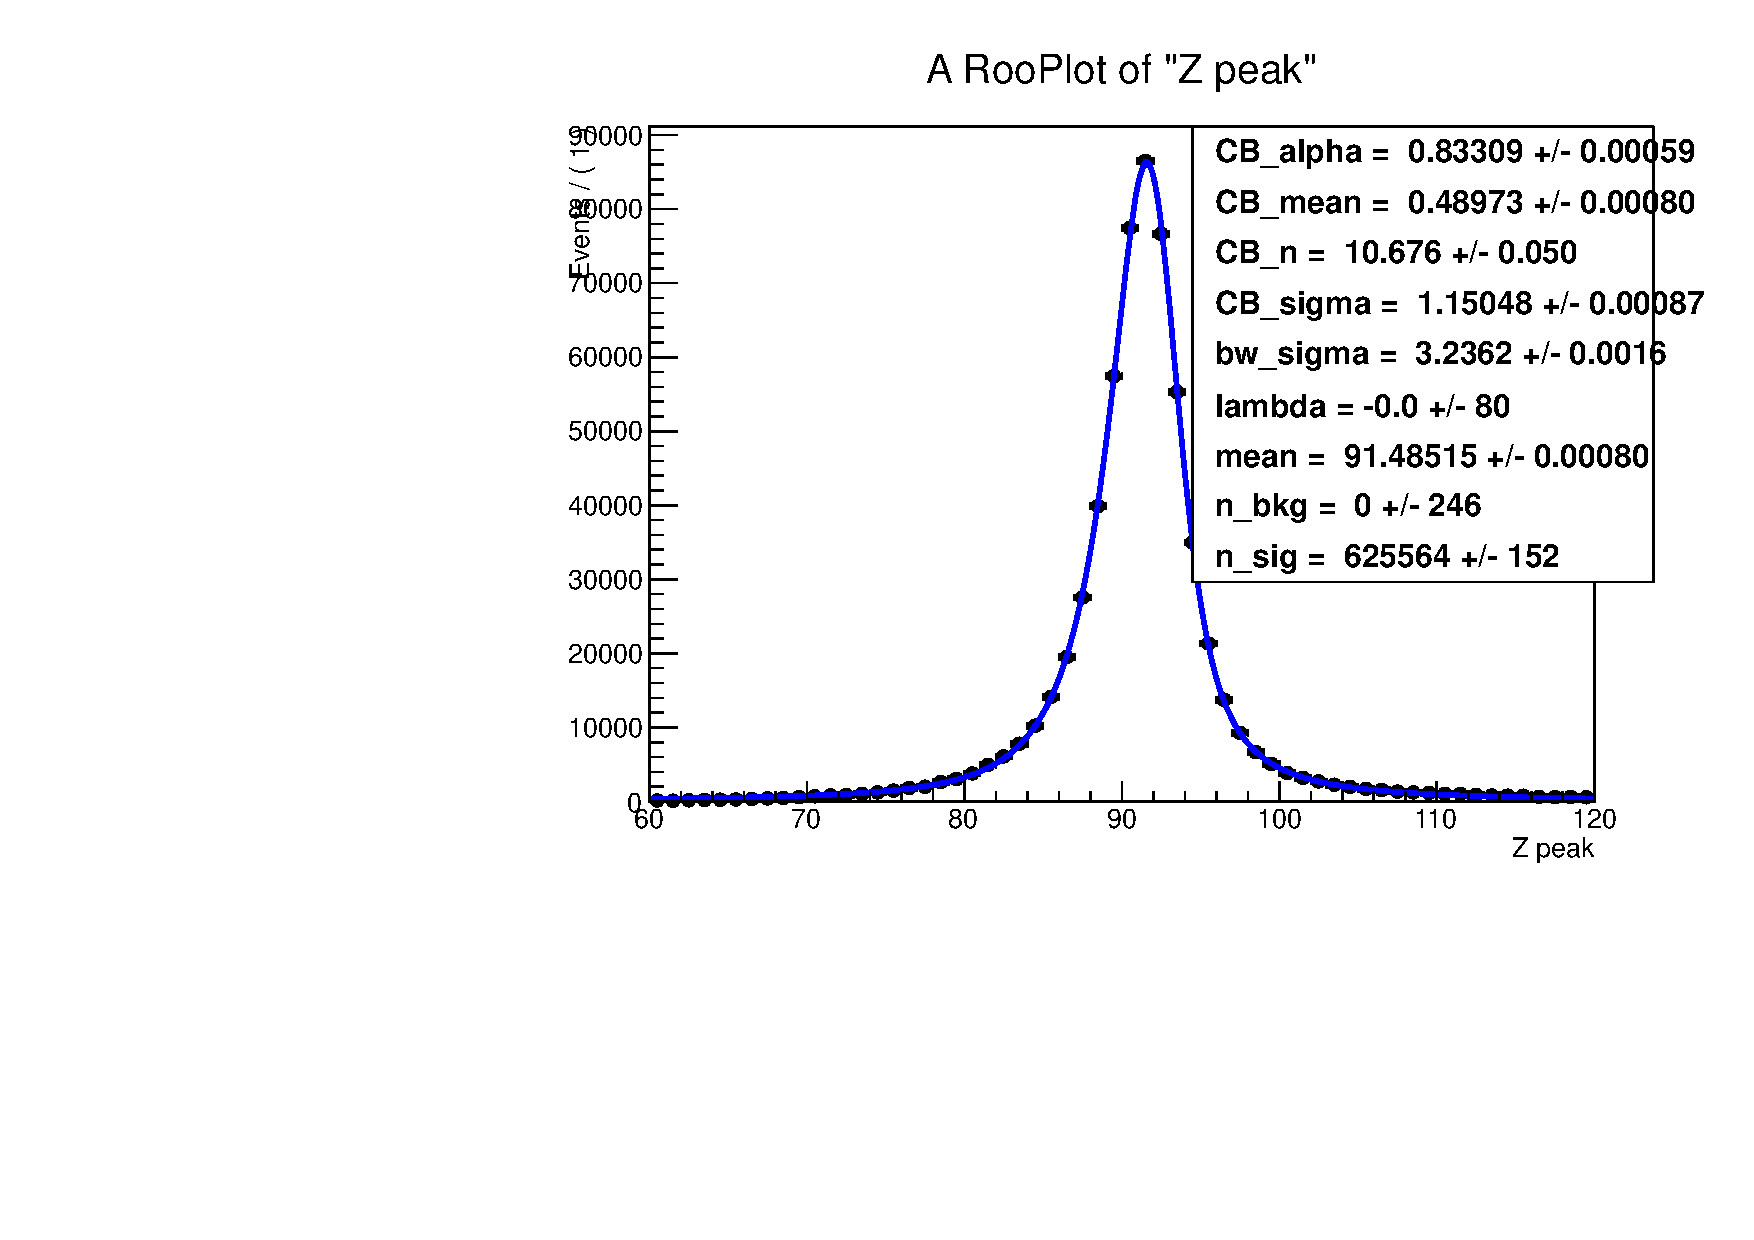
\includegraphics[width=0.48\textwidth]{Chapters/04_Analysis/04b_XSections/images/lepton_scale_factors/CBConvolution/electron/data/id_iso/tagProbe_total_Z_peak}\hfill
      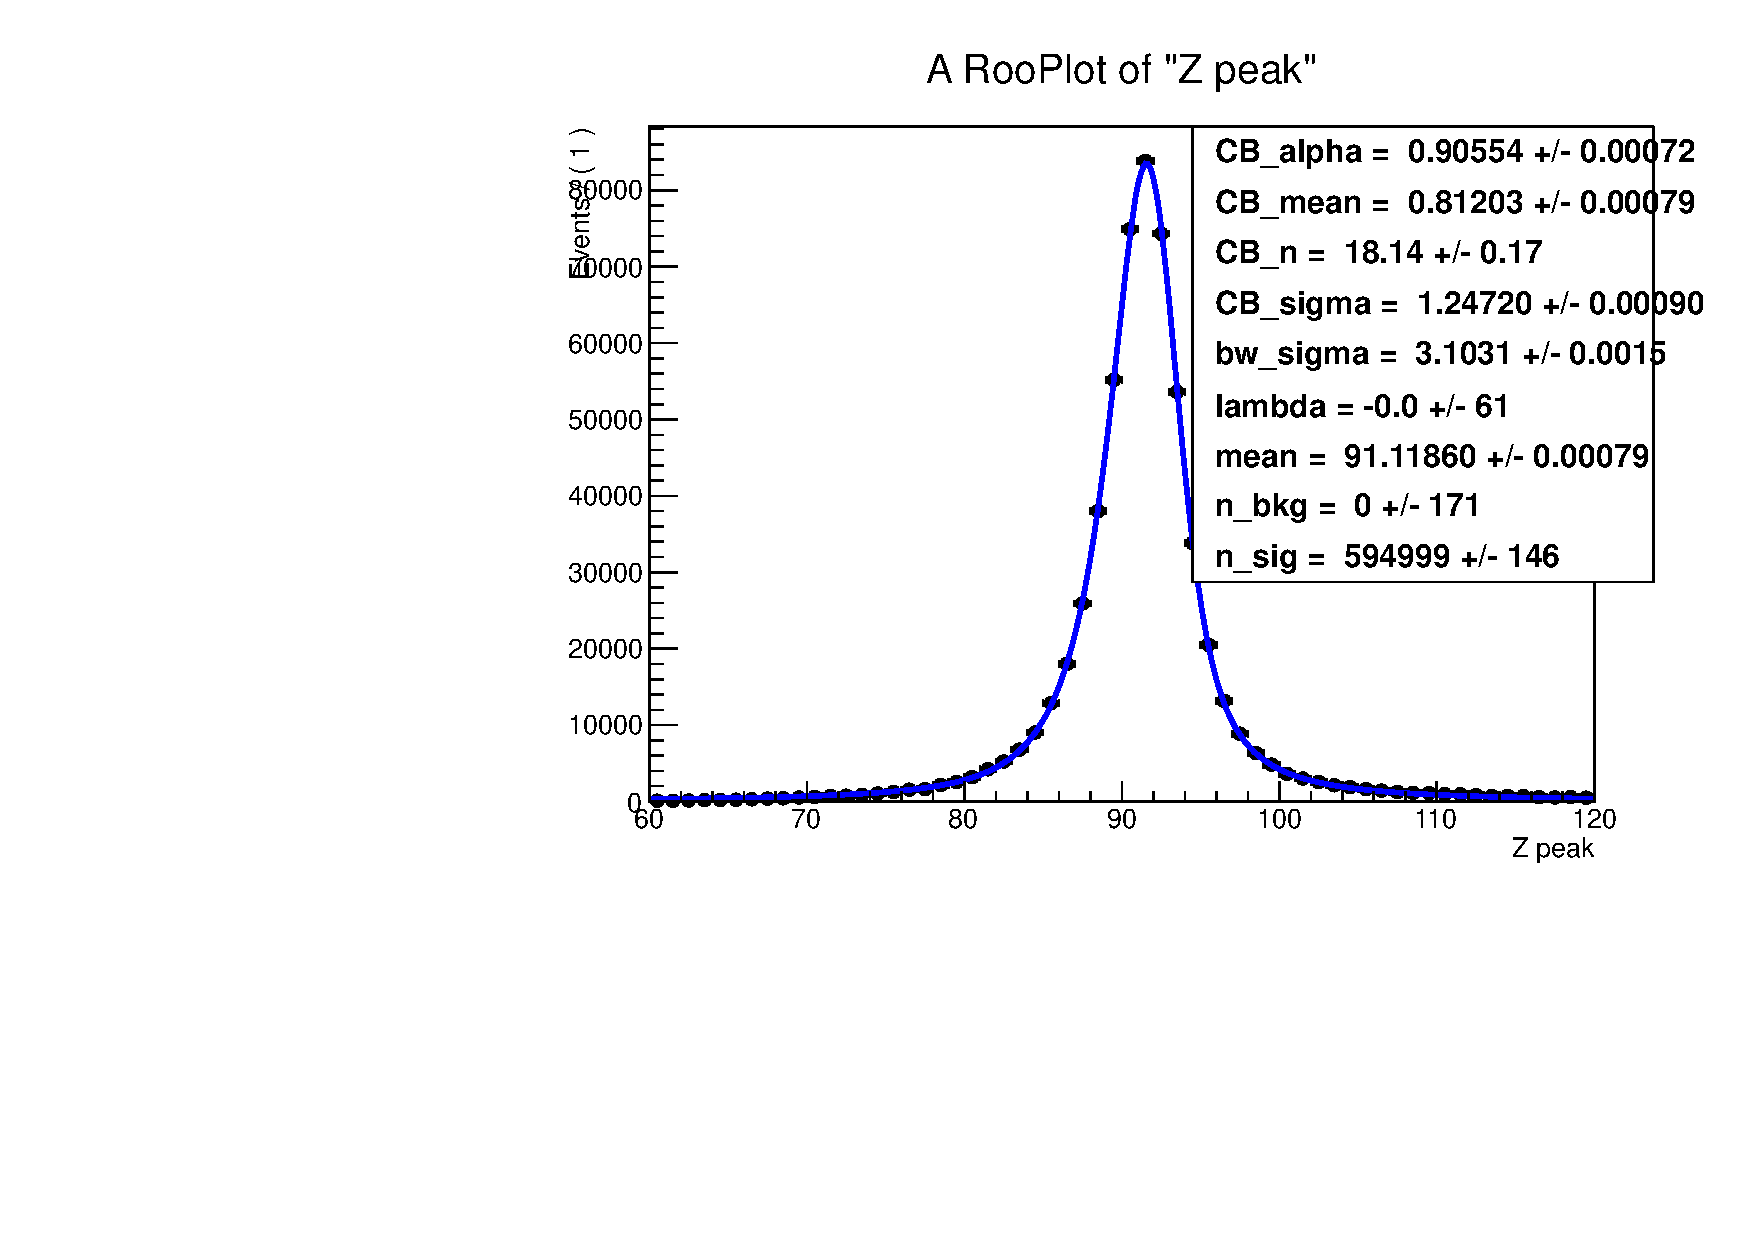
\includegraphics[width=0.48\textwidth]{Chapters/04_Analysis/04b_XSections/images/lepton_scale_factors/CBConvolution/electron/data/id_iso/tagProbe_passed_Z_peak}\\
     \caption{Fits of the invariant mass distribution of all tag-and-probe pairs (left) and for
     tag-and-probe pairs in which the probe satisfies the identification and isolation criteria
     (right).}
     \label{fig:electron_id_iso_efficiency_invariant_Z_mass_fits}
\end{figure}

The efficiency of the identification and isolation process is then calculated using the numbers extracted
from the fits, in bins of \pt and $\eta$ of the probe electron, as follows:

\begin{equation}
\epsilon(\text{identification and isolation}) = \frac{N^{\text{fit}}_{\text{probe, passing}}}{N^{\text{fit}}_{\text{probe, all}}}
\end{equation}

The scale factor is then calculated as the ratio between the efficiencies in simulation and in data. The
efficiencies in both can be seen to be similar in Figure~\ref{fig:electron_id_iso_efficiencies_wrt_eta_pt},
leading to scale factors close to one.

\begin{figure}[hbtp]
    \centering
      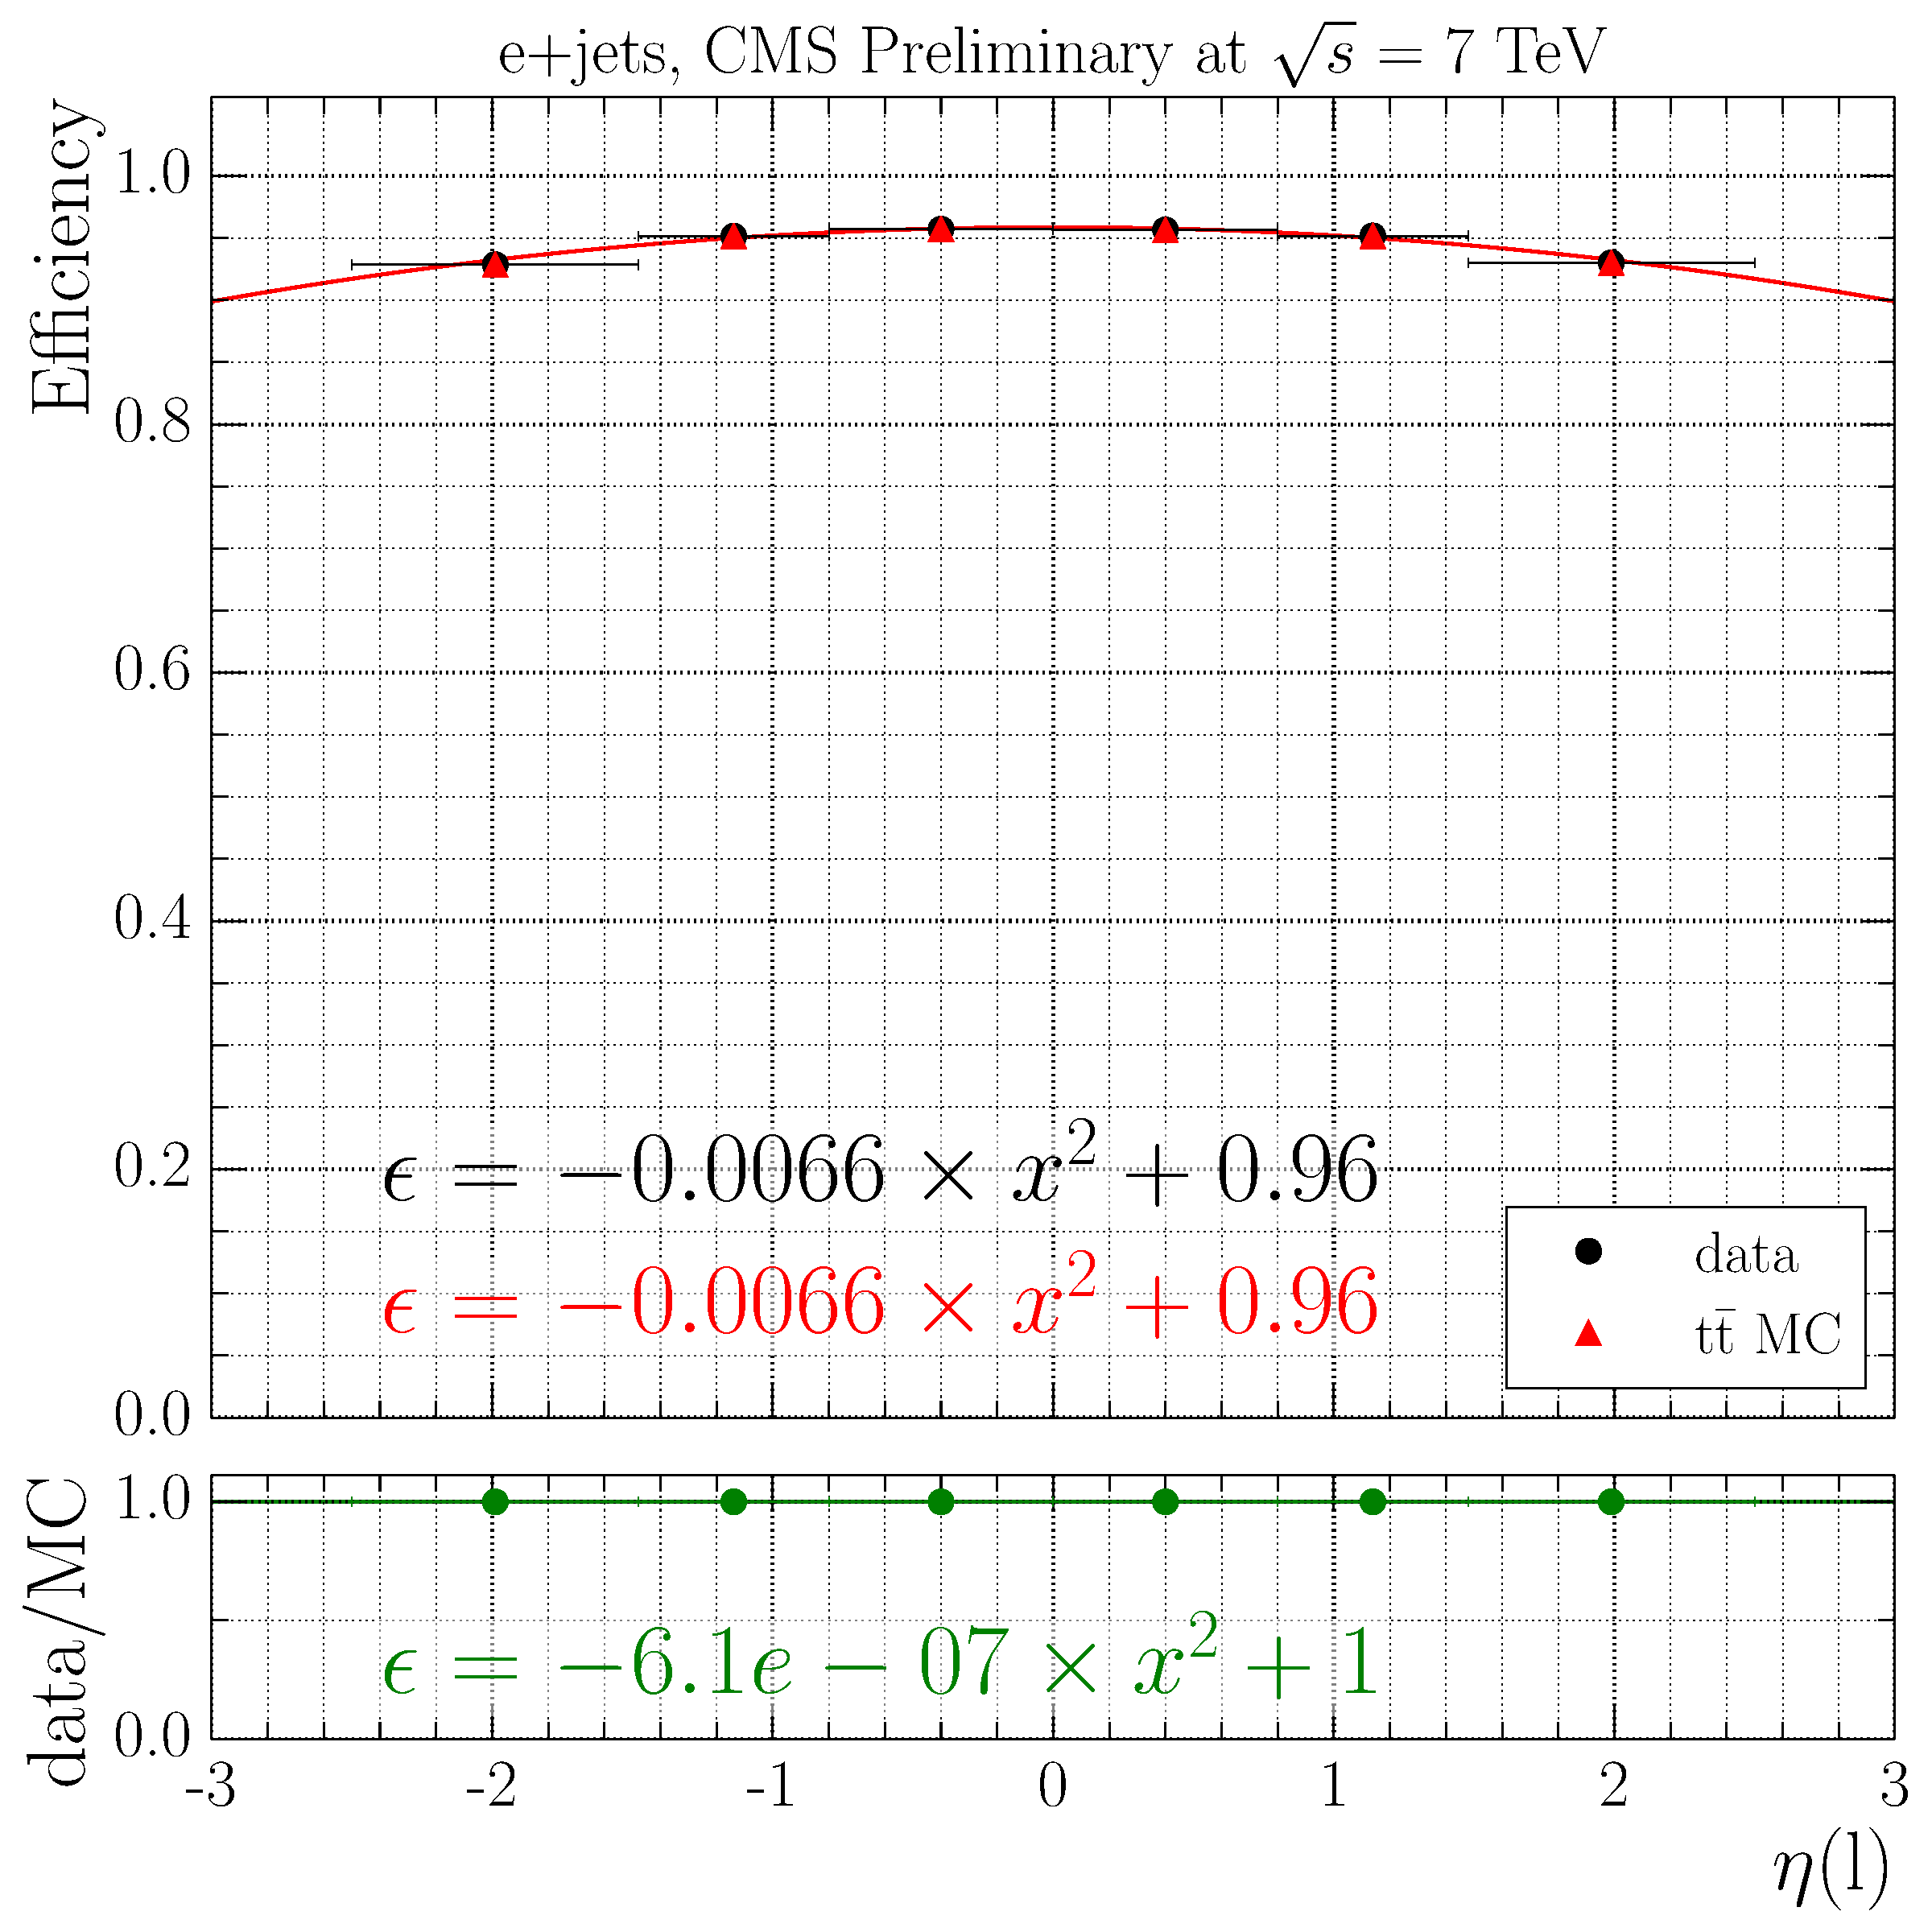
\includegraphics[width=0.48\textwidth]{Chapters/04_Analysis/04b_XSections/images/lepton_scale_factors/CBConvolution/electron/efficiency_eta_id_iso}\hfill
      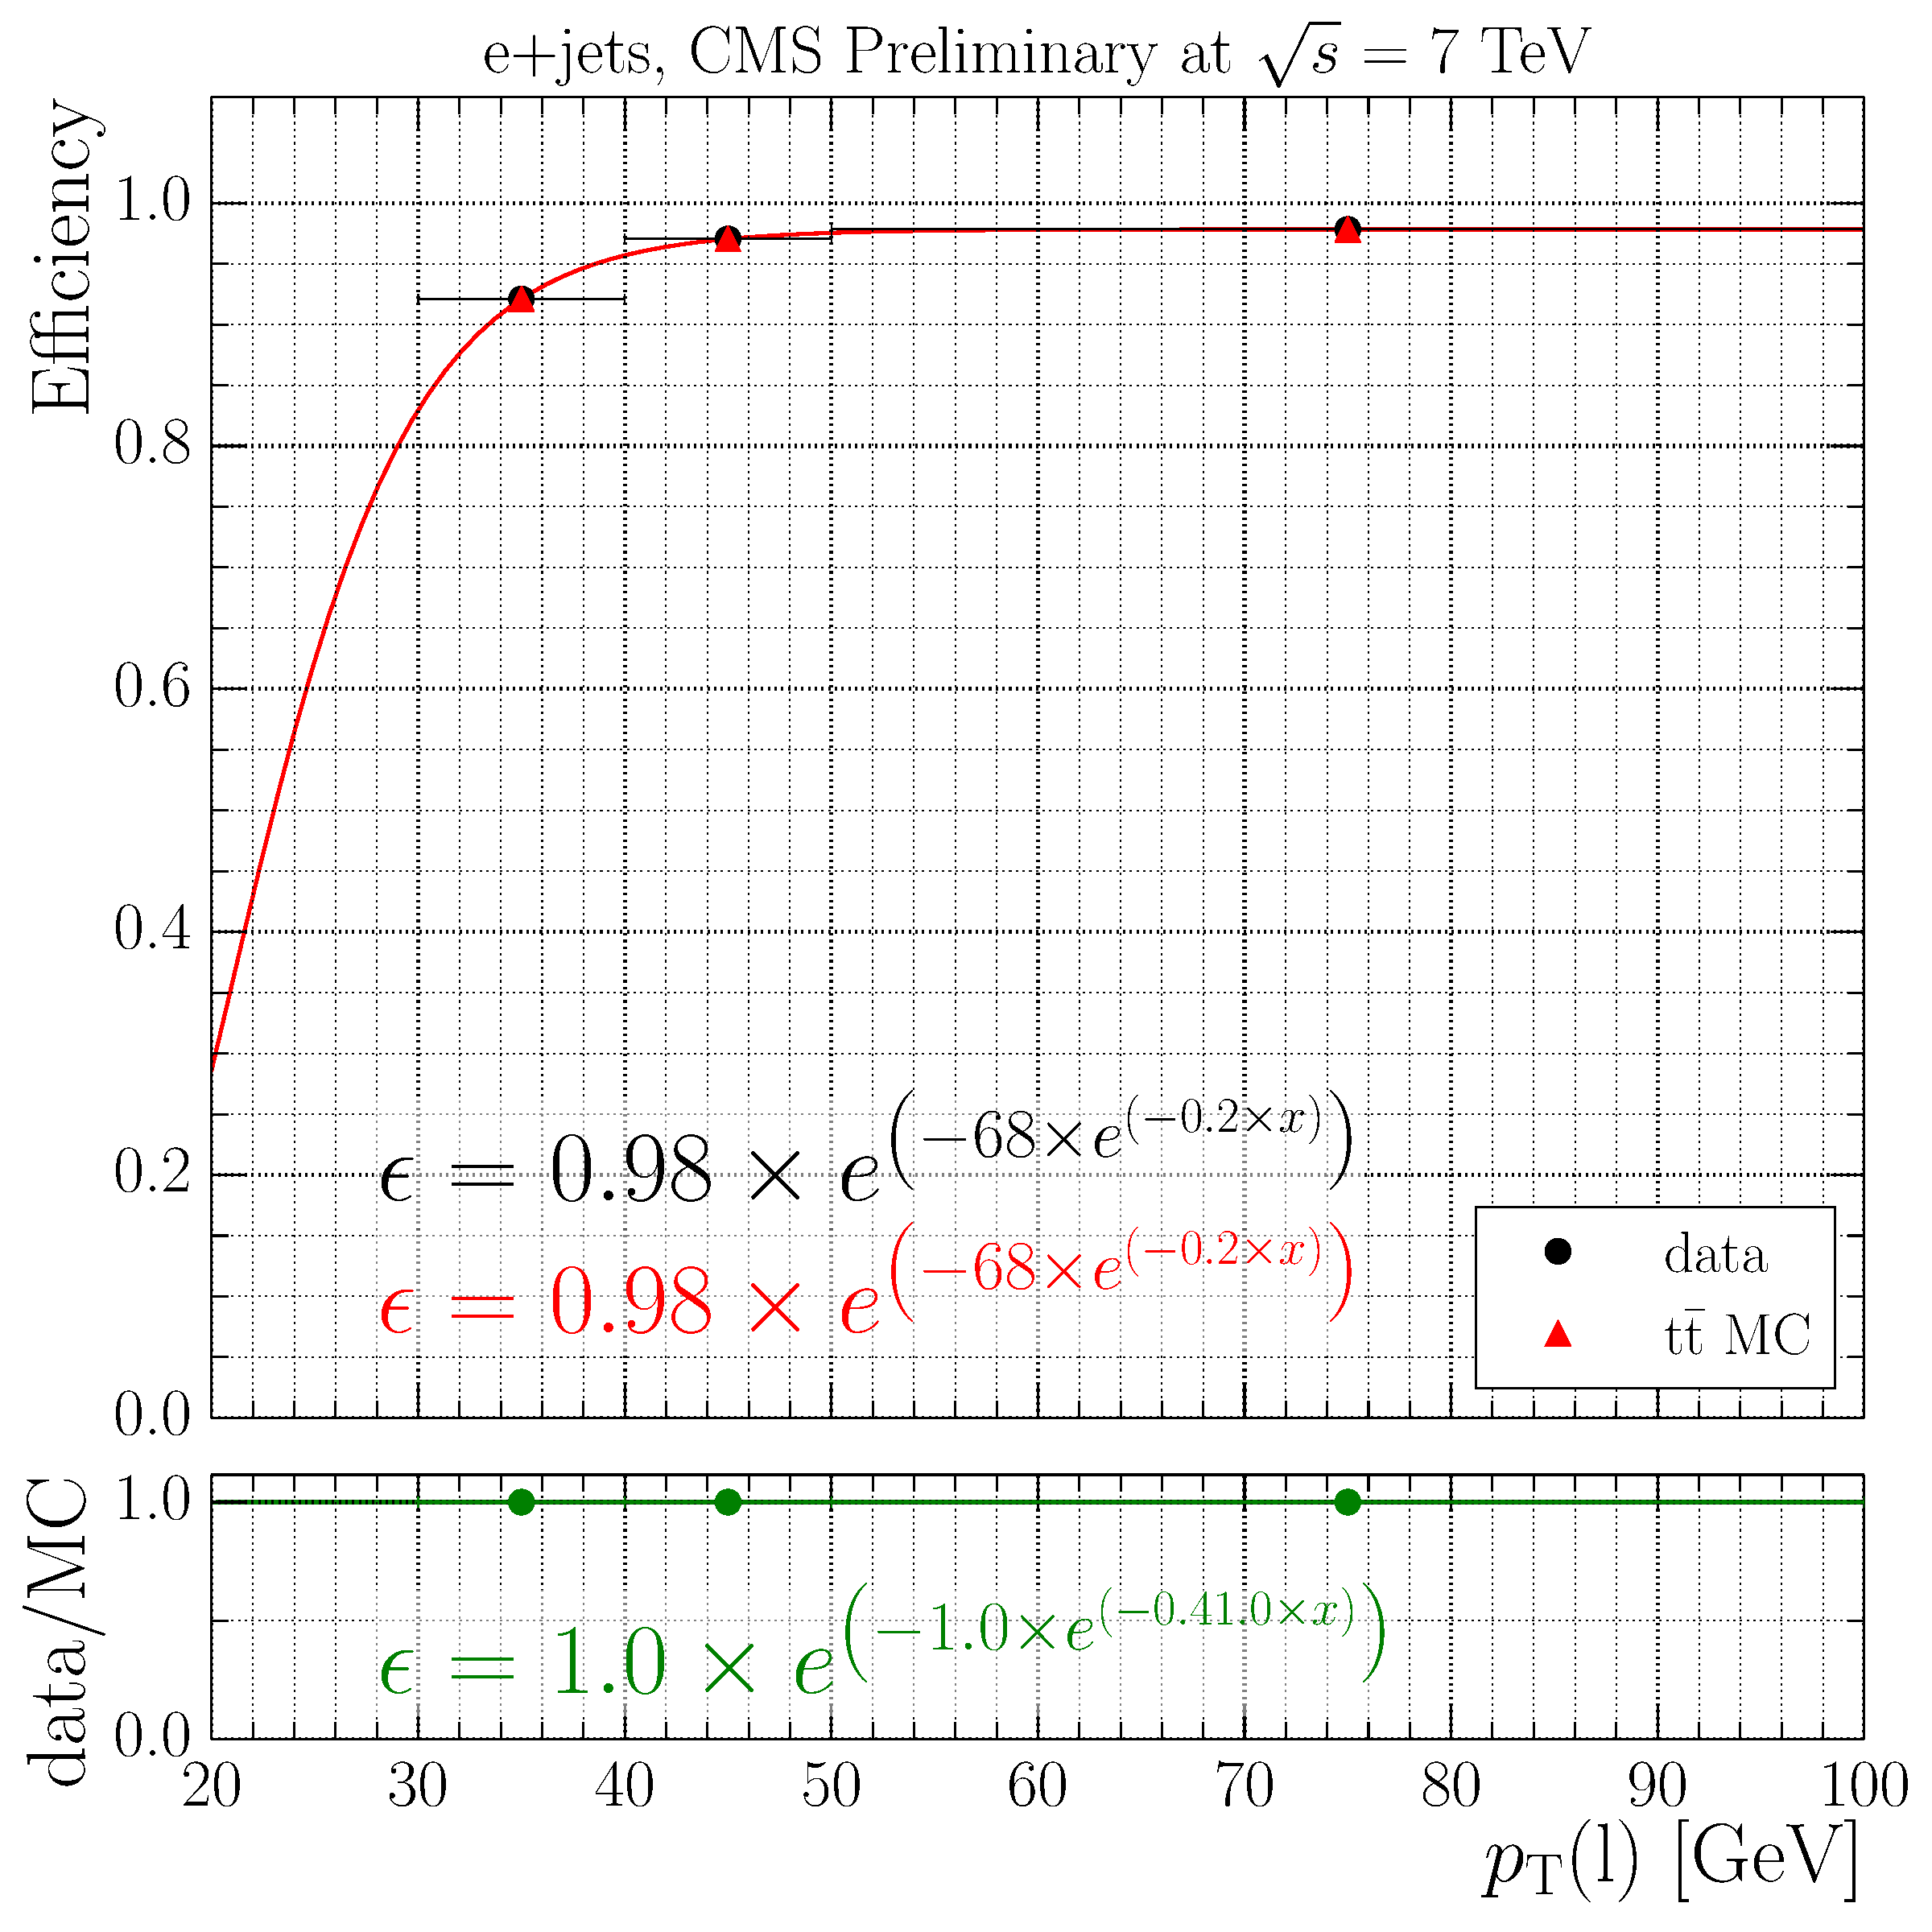
\includegraphics[width=0.48\textwidth]{Chapters/04_Analysis/04b_XSections/images/lepton_scale_factors/CBConvolution/electron/efficiency_pt_id_iso}
      \caption{Identification and isolation efficiencies as a function of $\eta$ and \pt in data and \ttbar
      Monte Carlo simulation.}
     \label{fig:electron_id_iso_efficiencies_wrt_eta_pt}
\end{figure}

The efficiency of the electron part of the trigger is then similarly calculated, with respect to the
identification and isolation requirements, meaning the events passing the identification and isolation
requirements in the previous stage are then used as the baseline for the trigger efficiency. The subset of
these in which the probe electron matches a HLT electron is then used to calculate the efficiency as follows:

\begin{equation}
\epsilon(\text{trigger}) = \frac{N^{\text{fit}}_{\text{probe, matching HLT}}}{N^{\text{fit}}_{\text{probe,identification and isolation}}}
\end{equation}

In order to calculate the efficiency of the hadron leg of the trigger, the full selection with only the
electron part of the trigger and without \btagging is taken as the baseline. The number of events passing the
hadronic leg of the trigger is then used to calculate the hadronic leg efficiency as follows:

\begin{equation}
\epsilon(\text{hadron leg}) = \frac{N_{\text{hadron leg, passing}}}{N_{\text{selected}}}
\end{equation}

The scale factors are produced in bins of \pt and $\eta$ of the fourth most energetic jet, since this is the
lowest energy jet that is selected. Parametrising as a function of higher energy jets would lead to a bias
towards high efficiencies as the trigger will have a higher efficiency at higher jet energies.

Equivalent fit and efficiency plots for the trigger are included in
Figures~\ref{fig:electron_trigger_efficiency_invariant_Z_mass_fits} and
\ref{fig:electron_trigger_efficiencies_wrt_eta_pt} in Appendix~\ref{as:data_monte_carlo_corrections}.
TODO:HAVE NOT INCLUDED MUON ID-ISO OR TRIGGER PLOTS ANYWHERE. HOPEFULLY OK WITH JUST ELECTRON PLOTS.
